\chapter{Introduction}
\label{ch:Introduction}

\section{Motivation \& Objective}
\label{sec:Motivation and Objective}

% visualisierung

Modifying resources by a specific property within the graph-based \acrfull*{RDF} can be an exhausting and expensive task. This is particularly the case when managing graph resources in plain text formats (e.g., in Turtle or \acrshort*{SPARQL}), as it requires trained people to maintain the data, and, despite their expertise, it would still be prone to human error. To overcome this challenge, much effort has been previously invested in developing possible solutions for managing graph data in a visual context. One solution to manage semantic and metadata is the software solution \textit{Corporate Memory} developed by eccenca GmbH in Leipzig, Germany. \textit{Corporate Memory} consists of three core components, namely (1) \textit{DataIntegration}, (2) \textit{DataPlatform}, and (3) \textit{DataManager}. The latter component provides a comprehensive visual representation of a knowledge base and allows intuitive authoring of semantic content.

The aim of the current thesis was to create a prototypical component for the \textit{DataManager}, that provides an approach to address the issue of modifying resources by a specific property in an intuitive way. The prototype (throughout the work also referred to as \textit{\acrlong*{RMB}} (\acrshort*{RMB})), addresses two main goals, that are documented in the current thesis: (1) visualizing a certain section of a knowledge graph (i.e., a subgraph) within a Kanban board, and (2) the possibility of modifying a specific property by dragging a resource into another column.

The following example captures the essence of both goals and illustrates the transformation process. \autoref{lst:MinimalGraph} illustrates a minimal \acrshort*{RDF} graph. In simple terms, the graph expresses that the material \textit{marble} has a \textit{color} that is set to \textit{white}.

\begin{spacing}{0.9}
    \lstset{language=JavaScript,escapechar=|}
    \begin{lstlisting}[
    label={lst:MinimalGraph},
    xleftmargin=18em, % this needs to be manually adjusted to center the frame
    xrightmargin=-18em, % this needs to be manually adjusted to center the frame
    caption={[A Minimal \tracknshrink{RDF} Graph]A minimal graph in \acrshort*{RDF}.}]
|<\url{http://dbpedia.org/page/Marble}>|
  |<\url{http://dbpedia.org/property/color}>|
    |<\url{http://dbpedia.org/page/White}> .|
\end{lstlisting}
\end{spacing}

\noindent Typically, (directed) graphs are visualized by a set of ellipses that are interconnected by arrows. Ellipses represent the graph’s nodes, while arrows describe the graph’s edges. \autoref{fig:White Marble Graph} visualizes \autoref{lst:MinimalGraph} as a directed graph:


\begin{figure}[ht]
    \libertineLF
    \centering
    

\tikzset{every picture/.style={line width=0.75pt}} %set default line width to 0.75pt        

\begin{tikzpicture}[x=0.75pt,y=0.75pt,yscale=-1,xscale=1]
%uncomment if require: \path (0,113); %set diagram left start at 0, and has height of 113

%Shape: Ellipse [id:dp21019483310286535] 
\draw  [draw opacity=0][fill={rgb, 255:red, 104; green, 139; blue, 181 }  ,fill opacity=1 ][blur shadow={shadow xshift=0pt,shadow yshift=-2.25pt, shadow blur radius=1.5pt, shadow blur steps=4 ,shadow opacity=25}] (162,54.41) .. controls (162,42.19) and (187.63,32.29) .. (219.25,32.29) .. controls (250.87,32.29) and (276.5,42.19) .. (276.5,54.41) .. controls (276.5,66.62) and (250.87,76.52) .. (219.25,76.52) .. controls (187.63,76.52) and (162,66.62) .. (162,54.41) -- cycle ;
%Straight Lines [id:da920285236062053] 
\draw [color={rgb, 255:red, 104; green, 139; blue, 181 }  ,draw opacity=1 ][line width=3]    (286.5,54.41) -- (358.5,54.41) ;
\draw [shift={(363.5,54.41)}, rotate = 180] [fill={rgb, 255:red, 104; green, 139; blue, 181 }  ,fill opacity=1 ][line width=3]  [draw opacity=0] (18.75,-9.01) -- (0,0) -- (18.75,9.01) -- (12.45,0) -- cycle    ;

%Shape: Ellipse [id:dp39386286974940465] 
\draw  [draw opacity=0][fill={rgb, 255:red, 104; green, 139; blue, 181 }  ,fill opacity=1 ][blur shadow={shadow xshift=0pt,shadow yshift=-2.25pt, shadow blur radius=1.5pt, shadow blur steps=4 ,shadow opacity=25}] (373.5,54.41) .. controls (373.5,42.19) and (399.13,32.29) .. (430.75,32.29) .. controls (462.37,32.29) and (488,42.19) .. (488,54.41) .. controls (488,66.62) and (462.37,76.52) .. (430.75,76.52) .. controls (399.13,76.52) and (373.5,66.62) .. (373.5,54.41) -- cycle ;

% Text Node
\draw (430.75,54.41) node {{{\large \textsf{\textbf{:White}}}}};
% Text Node
\draw (219.25,54.41) node {{{\large \textsf{\textbf{:Marble}}}}};
% Text Node
\draw (317.75,43.41) node {{\textsf{\textbf{:color}}}};


\end{tikzpicture}

    \caption[Minimal Graph Visualization]{A minimal graph visualizing \autoref{lst:MinimalGraph}.}
    \label{fig:White Marble Graph}
    \libertineOsF
\end{figure}


\noindent In the previous example, the graph’s property is \textit{color}, and its current value is a resource that refers to \textit{white}. In order to change the value of the property from white to red, the graph could be manually modified, for example, by a \acrshort*{SPARQL} query. However, as mentioned above, this approach is prone to error in many ways.

\newpage

\noindent In basic terms, this work merges the concept of \acrshort*{RDF} with the concept of a Kanban board. Specifically, a particular portion of an \acrshort*{RDF} graph will be selected and mapped into a Kanban board. Furthermore, from that portion, a particular property will be selected to represent the columns of the board. Finally, the board will allocate its content (i.e., resources) over these columns.


\autoref{fig:White Marble Kanban Board} depicts a mockup version of a Resource Management Board. In addition to the data from the previous example, this illustration contains one more resource (i.e., the material copper) and embeds both elements in a broader domain (i.e., a material database, which is also used as the board’s title). Since \textit{color} was selected as the preferred column property, the contents of the board have been structured accordingly. This means that all resources are grouped by their inherent color property. Therefore, the resource marble was initially placed in the column labeled white. In contrast to \autoref{fig:White Marble Graph}, the visual projection of graph data, as seen in \autoref{fig:White Marble Kanban Board}, is a novel approach for semantic data exploration.

In addition to visualize graph data, the second goal of this thesis is the modification of a property’s value by dragging a resource into another column. To illustrate this goal, the resources in \autoref{fig:White Marble Kanban Board} (i.e., marble and copper) are depicted as draggable cards that can be moved arbitrarily over the columns of the board. As depicted by the arrow, the card holding the resource for marble is getting dragged from the first to the second column. Eventually, when dropping the card to its target column, an update on the underlying graph gets triggered, which will assign the corresponding column value (i.e., red) to that specific property (i.e., color) on that particular resource (i.e., marble). Using the drag and drop capabilities of a Kanban board to manage specific properties of a resource is a novel and user-friendly approach to manage knowledge data. Without requiring profound expertise in the field of \tns{RDF}, it enables users to easily and intuitively manage complex graph structures.

\begin{figure}[ht]
    \libertineLF
    \centering
    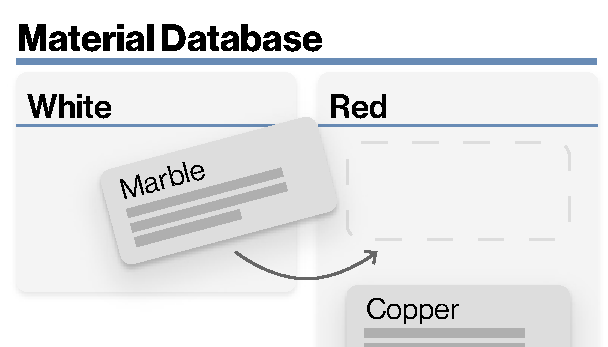
\includegraphics[width=73mm]{img/12-RMB-Mockup.pdf}
    \caption[Mockup of the Resource Management Board]{Mockup of the Resource Management Board.}
    \label{fig:White Marble Kanban Board}
    \libertineOsF
\end{figure}



\section{Structure of This Work}
\label{sec:structure}

This thesis is structured as follows. First, \autoref{ch:Background} provides a theoretical background for the two main concepts involved in this work: (1) Semantic Web with the focus on the \acrshort*{RDF} and (2) Kanban. Then, \autoref{ch:Requirements} introduces four use cases and derives corresponding functional and non-functional requirements. Thereupon, \autoref{ch:State of the Art} presents an overview of existing  Kanban board solutions and evaluates them with regard to the desired requirements. Hereafter, \autoref{ch:Specifications} provides specifications for the prototype, including the target data model and query strategy. In \autoref{ch:Implementation}, the corresponding implementation is outlined in detail. Lastly, \autoref{ch:Discussion} provides an overall evaluation of this implementation, based on the outlined requirements. Moreover, the limitations of the current status of the prototype will be discussed, together with possible future directions. 
